\section{Appendix}

\subsection{The duplex construction}

\begin{figure}[htbp]
  \centering
  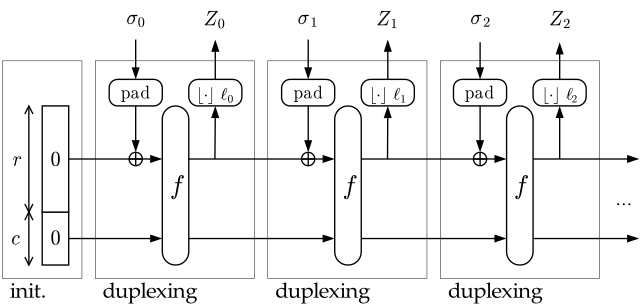
\includegraphics[width=0.5\textwidth]{images/Duplex-150.png}
  \caption{The duplex construction.}
  \label{fig:duplex}
\end{figure}

An alternation of the sponge construction is the \textbf{duplex construction}. Permutation function $f$, padding function $P$ and parameter bitrate $r$ are also used in the duplex construction, while $\sigma$ is the input string and $\ell$ is the requested number of bits. \cite{keccak_team,sponge_function_2023,guido_b_d_michaël_p_2011} \par 

While the sponge function is stateless between calls, the duplex version alternates between absorbing data into the state and squeezing data out of the state, where the output depends on all the previous inputs. \cite{guido_b_d_michaël_p_2011,cryptoeprint:2023/796} During the absorption phase, input data is XORed with the rate part of the state and then permuted using the permutation function. During the squeezing phase, output data is obtained by reading from the rate part of the state while keeping the capacity part fixed. \par